% Section: choice of the deferral penalty (Yoon).
% Needs \usepackage{graphicx}. Figures come from pddl/lambda-sweep/figures.py
% (copied to report/figures/).

\subsection{Choosing the deferral penalty}
\label{sec:lambda}

Every person must end the plan either delivered to an evacuation point or deferred to a later
rescue wave. Following the compilation of soft goals into action costs of Keyder and
Geffner~\cite{keyder2009soft}, deferring a person of band $b$ costs a penalty $p_b$ in the same
unit as driving (minutes), and the planner minimises
\[
  \text{cost} \;=\; \sum_{\text{drives}} t(e) \;+\; \sum_{\text{deferred people}} p_b .
\]
We write the penalty as a product of two parts that can each be justified on their own:
\[
  p_b = \lambda \cdot r_b, \qquad
  r_{\text{injured}} = 4,\; r_{\text{child}} = 3,\; r_{\text{elderly}} = 2.5,\; r_{\text{adult}} = 1 .
\]
The urgency weights $r_b$ fix the \emph{order} of priority, taken from triage practice
(injured first, then children, then the elderly, then adults), relative to an adult. The
scale $\lambda$ is an exchange rate: the number of driving minutes the team is willing to
spend to rescue one adult now rather than leave them for the next wave. Roughly, an optimal
plan rescues a group when the extra driving needed to fetch them is less than the penalties
$\lambda r_b$ it would otherwise pay. We use $\lambda = 20$, which gives penalties of 80, 60, 50 and 20 minutes.

\paragraph{Why $\lambda$ matters.}
$\lambda$ decides what kind of problem the benchmark is. At $\lambda = 0$ deferring is free and
the optimal plan defers everyone without moving. When $\lambda$ is large, deferring is never
worth it, every reachable person is rescued, and the problem becomes pure capacitated vehicle
routing with no triage left in it. (Minimising the number of people deferred first and only then
the driving, a lexicographic objective we also considered, behaves like this
large-$\lambda$ limit.) The
interesting regime, where the planner has to decide \emph{who} to leave behind, lies in
between. To find it we re-solved all 45 instances to optimality with \texttt{exact.py}
(Section~\ref{sec:exact}) for $\lambda \in \{0, 5, 10, 15, 20, 30, 40, 60, 80, 120\}$,
keeping $r_b$ fixed. People whom no car can reach because of damaged roads are deferred at
every $\lambda$, so we leave them out of the counts below.

\begin{figure}[t]
  \centering
  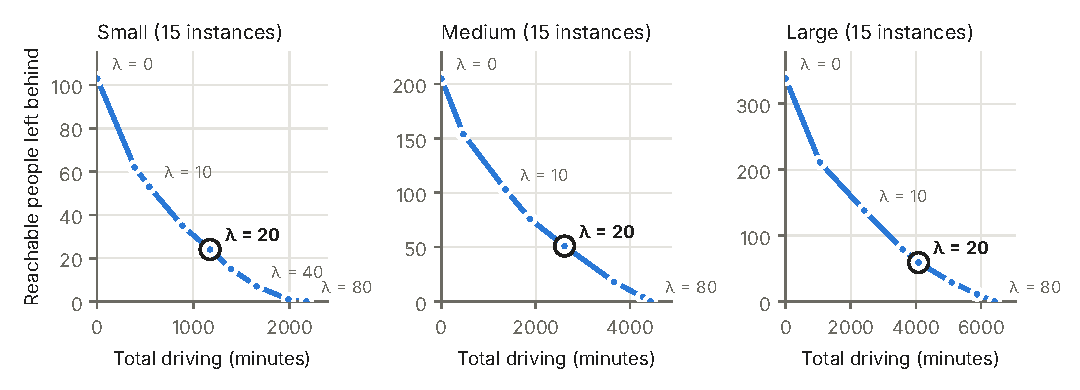
\includegraphics[width=\linewidth]{figures/tradeoff.pdf}
  \caption{Trade-off between total driving and reachable people left behind, one point per
  value of $\lambda$ (sum over the 15 instances of each size; every point is a proven
  optimum). $\lambda = 20$, used in all our experiments, is circled.}
  \label{fig:tradeoff}
\end{figure}

\begin{figure}[t]
  \centering
  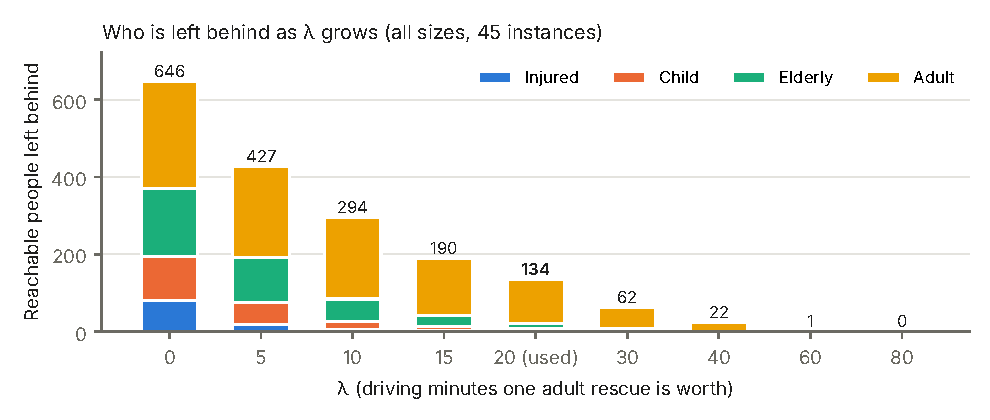
\includegraphics[width=0.92\linewidth]{figures/who-left.pdf}
  \caption{Reachable people left behind by band as $\lambda$ grows, over all 45 instances.
  The urgency weights $r_b$ are fixed; only the scale $\lambda$ changes.}
  \label{fig:who-left}
\end{figure}

\paragraph{What the sweep shows.}
Figure~\ref{fig:tradeoff} has the same shape for all three sizes: a convex curve where each
extra person rescued costs more driving than the last. Going from $\lambda = 10$ to $20$
rescues 160 more people for about 3{,}550 extra minutes of driving (about 22 minutes each);
going from $20$ to $40$ rescues 112 more for about 3{,}940 minutes (about 35 minutes each).
From $\lambda = 60$ upwards almost everyone reachable is rescued (one child in one small
instance remains at $\lambda = 60$, none at $\lambda = 80$) and the curve stops moving.

At $\lambda = 20$ the plans rescue 512 of the 646 reachable people (79\%) using 60\% of the
driving needed to rescue all of them, so the instances still require real triage decisions.
Figure~\ref{fig:who-left} shows that those decisions follow the intended priorities: of the
134 people left behind, 113 (84\%) are adults, 13 elderly, 7 children and 1 injured person
(on a large instance, where reaching them costs more than the 80-minute penalty). As
$\lambda$ grows the bars shrink in priority order: no reachable injured person is left from
$\lambda = 30$, no elderly person from $\lambda = 40$ and no adult from $\lambda = 60$. The
one exception is a single child in one small instance whose rescue needs between 180 and 240
minutes of extra driving, so they are rescued only from $\lambda = 80$.

We chose $\lambda = 20$ for three reasons. It lies in the middle of the trade-off curve on every
size, so instances are neither trivial (defer everyone, or rescue everyone) nor dominated by
one regime. It is the regime that tests what we want to compare: whether an LLM, planning
directly or through PDDL, makes the same who-to-leave decisions as the optimum. And at this
value the plans the planner prefers are ones a human coordinator would recognise, since the
people left behind are overwhelmingly the least urgent. All main results use $\lambda = 20$;
other values appear only in this analysis.

\paragraph{Limitations and responsible use.}
$\lambda$ and $r_b$ encode a value judgement, how much driving a rescue is worth and how much
more a child is worth than an adult, and our numbers are modelling choices rather than values
from disaster-management practice. The formulation makes that judgement explicit and
adjustable, which is a strength over leaving it implicit in an LLM's reasoning: an operator
can see exactly what $\lambda$ trades away, and Figure~\ref{fig:tradeoff} shows the
consequences of other choices. In a real deployment $\lambda$ and $r_b$ should be set and
signed off by the responsible humans, not tuned by the system, and a deferred person should be
read as ``rescued by the next wave'', not abandoned. Our model also has no clock, so it cannot
express that waiting longer is worse for the injured than for others; a time-dependent penalty
would capture this but makes the problem much harder to solve exactly.
